\documentclass[11pt,a4paper]{article}

\usepackage[margin=2.2cm]{geometry}
\usepackage{booktabs}
\usepackage{longtable}
\usepackage{array}
\usepackage{xcolor}
\usepackage{amsmath,amssymb}
\usepackage{enumitem}
\usepackage{caption}
\usepackage{listings}
\usepackage{tikz}
\usetikzlibrary{arrows.meta,positioning,fit,backgrounds,shapes.geometric,calc}
\usepackage[hidelinks]{hyperref}
\usepackage{microtype}
\usepackage{titlesec}

\definecolor{navy}{HTML}{1F3A5F}
\definecolor{teal}{HTML}{2C6E6A}
\definecolor{amber}{HTML}{B7791F}
\definecolor{soft}{HTML}{F4F6F8}
\definecolor{rule}{HTML}{D5DBE1}

\titleformat{\section}{\Large\bfseries\color{navy}}{\thesection}{0.6em}{}
\titleformat{\subsection}{\large\bfseries\color{teal}}{\thesubsection}{0.5em}{}
\titleformat{\subsubsection}{\normalsize\bfseries}{\thesubsubsection}{0.4em}{}

\lstset{
  basicstyle=\ttfamily\scriptsize,
  breaklines=true,
  columns=fullflexible,
  keepspaces=true,
  frame=single,
  rulecolor=\color{rule},
  backgroundcolor=\color{soft},
  showstringspaces=false,
  upquote=true,
  aboveskip=6pt,
  belowskip=6pt
}

\newcommand{\code}[1]{\texttt{\small #1}}
\newcommand{\key}[1]{\textbf{#1}}
\setlength{\parskip}{3pt}
\setlength{\parindent}{0pt}

\title{\vspace{-1.2cm}\textbf{\color{navy}Glass-box Rare-Disease Retrieval and\\Evidence-Grounded Explanation}\\[0.3em]
\large Architecture, training, evaluation, and live-deployment handoff}
\author{ZebraMap benchmark -- fusion v4 SHAP-8 system}
\date{23 November 2026 \quad version 1.0}

\begin{document}
\maketitle

\begin{center}
\fbox{\parbox{0.93\textwidth}{\small
\textbf{Purpose of this document.} This is the complete handoff for building a live
rare-disease agent on top of a frozen retriever. It documents the data split, text
preprocessing, retrieval models, trained weights, the multi-call explanation layer,
the exact prompts, evaluation results, and a recommended backend/frontend design
with conversation history.\\
\textbf{Status.} The retrieval system is validated on the full 10,702-case test set.
The LLM explanation layer is validated on a 62-case interim sample; its ranking
effect is mixed and is reported honestly in Section~\ref{sec:agent-results}.}}
\end{center}

\tableofcontents

\newpage
\section{Executive summary}

The system has two clearly separated parts.

\begin{enumerate}[leftmargin=1.4em]
\item \textbf{A frozen, deterministic retriever} that maps a case report to a
ranked list of 1,464 rare diseases. It combines a TF-IDF/SGD candidate retriever,
a mass80 BoW disease-centroid retriever, a 32-dimensional SVD representation, and a
LightGBM LambdaRank reranker. The final score is a fixed convex blend of the BoW
full-catalog score and the GBM pool score.
\item \textbf{An evidence-grounded explanation layer} that never changes the
candidate set. It extracts atomic case findings, fetches ZebraMap/Orphanet profile
sentences and OptimusKG triples deterministically, audits the ten candidates with
the retriever ranks hidden, writes cited claims for the final top five, validates
every citation, and adjudicates each claim as keep/soften/drop.
\end{enumerate}

\key{Validated retrieval performance} (full test set, 10,702 cases, 1,464-disease
catalog):

\begin{center}
\begin{tabular}{lrrrrr}
\toprule
System & MRR & Top-1 & Top-5 & Top-10 & R@100\\
\midrule
TF-IDF top-100 & 0.4203 & -- & 0.5344 & 0.6113 & 0.8213\\
BoW mass80 centroid & 0.4695 & -- & 0.5871 & 0.6533 & 0.8367\\
GBM full 115 & 0.4602 & -- & 0.5837 & 0.6574 & 0.8213\\
GBM v4 140 & 0.4614 & -- & 0.5933 & 0.6663 & 0.8213\\
Fusion v4 min--max & 0.4955 & -- & 0.6180 & 0.6824 & 0.8444\\
\textbf{Fusion v4 SHAP-8 (shipped)} & \textbf{0.4960} & \textbf{0.3911} & \textbf{0.6199} & \textbf{0.6848} & \textbf{0.8437}\\
\bottomrule
\end{tabular}
\end{center}
{\footnotesize All values are full-test-set results. Top-1 is reported only for the
shipped model; the other systems were evaluated on MRR and recall cutoffs.}

\key{Agent-layer finding (interim, 62 cases, Gemma-4-E4B).} The LLM audit
\emph{improves} cases whose gold disease was ranked 2--5 by the retriever
(MRR 0.378 $\rightarrow$ 0.612) but \emph{harms} correct top-1 cases
(1.000 $\rightarrow$ 0.707). Net MRR change is $-0.055$ (95\% CI $-0.138$ to $+0.028$).
The LLM-only baseline, which sees the same ten candidates without evidence, is also
below retrieval. Therefore the recommended production default is:
retriever ranking + grounded evidence display; treat LLM reordering as an optional,
user-toggleable feature until a stronger model or a rank-prior blend is validated.

\key{What is in the handoff folder.}
\begin{itemize}[leftmargin=1.4em]
\item \code{weights/retriever/} -- every weight needed to reproduce the shipped
retriever from raw text, including a reference implementation that matches the
cached top-10 exactly.
\item \code{weights/catalog/} -- disease index, full ZebraMap/Orphanet profiles, and
a compact OptimusKG slice for all 1,464 catalog diseases.
\item \code{code/} -- the end-to-end multi-call pipeline, the reference retriever,
the prompt appendix, and a backend skeleton.
\item \code{results/} -- full-test retrieval metrics and the interim agent evaluation.
\item \code{docs/} -- this document (LaTeX source and PDF).
\end{itemize}

\section{System at a glance}

\begin{figure}[h]
\centering
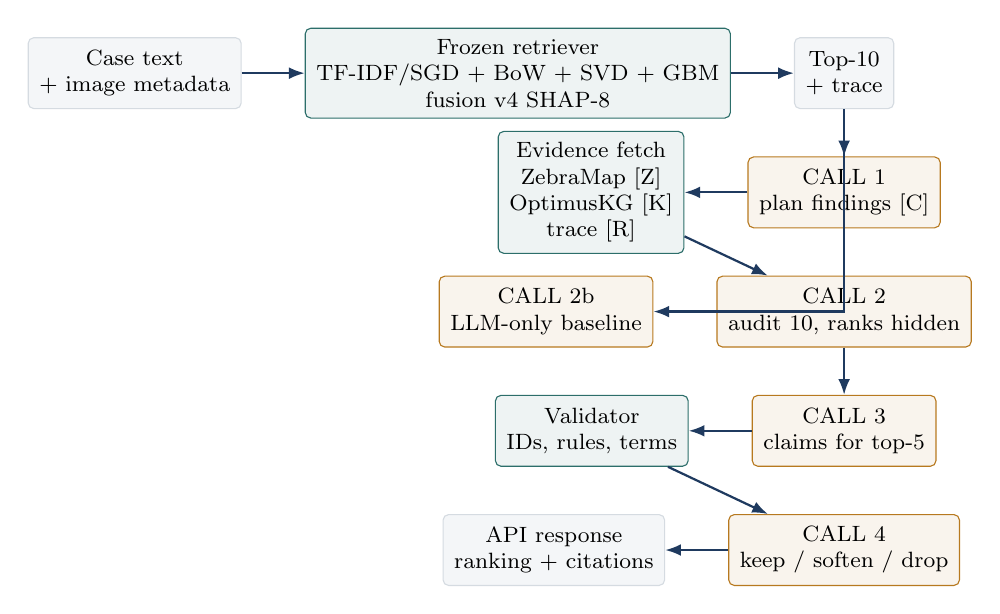
\begin{tikzpicture}[
  node distance=6mm and 8mm,
  box/.style={draw=rule,rounded corners=2pt,fill=soft,align=center,
              font=\footnotesize,inner sep=4pt,minimum height=9mm},
  llm/.style={draw=amber,rounded corners=2pt,fill=amber!8,align=center,
              font=\footnotesize,inner sep=4pt,minimum height=9mm},
  det/.style={draw=teal,rounded corners=2pt,fill=teal!8,align=center,
              font=\footnotesize,inner sep=4pt,minimum height=9mm},
  arr/.style={-{Latex[length=2mm]},draw=navy,thick}
]
\node[box] (case) {Case text\\+ image metadata};
\node[det,right=of case] (ret) {Frozen retriever\\TF-IDF/SGD + BoW + SVD + GBM\\fusion v4 SHAP-8};
\node[box,right=of ret] (top) {Top-10\\+ trace};
\node[llm,below=of top] (plan) {CALL 1\\plan findings [C]};
\node[det,left=of plan] (ev) {Evidence fetch\\ZebraMap [Z]\\OptimusKG [K]\\trace [R]};
\node[llm,below=of plan] (audit) {CALL 2\\audit 10, ranks hidden};
\node[llm,left=of audit] (only) {CALL 2b\\LLM-only baseline};
\node[llm,below=of audit] (write) {CALL 3\\claims for top-5};
\node[det,left=of write] (val) {Validator\\IDs, rules, terms};
\node[llm,below=of write] (adj) {CALL 4\\keep / soften / drop};
\node[box,left=of adj] (rep) {API response\\ranking + citations};
\draw[arr] (case) -- (ret);
\draw[arr] (ret) -- (top);
\draw[arr] (top) -- (plan);
\draw[arr] (plan) -- (ev);
\draw[arr] (ev) -- (audit);
\draw[arr] (top) |- (only);
\draw[arr] (audit) -- (write);
\draw[arr] (write) -- (val);
\draw[arr] (val) -- (adj);
\draw[arr] (adj) -- (rep);
\end{tikzpicture}
\caption{End-to-end architecture. Teal boxes are deterministic; amber boxes are LLM
calls. The retriever is frozen and never sees evidence. The LLM never controls
retrieval, never fetches data itself, and never introduces a new disease candidate.}
\label{fig:arch}
\end{figure}

The design commits to four rules:

\begin{enumerate}[leftmargin=1.4em]
\item \key{Retrieval is frozen.} No LLM output can add or remove a candidate from
the retriever's top-10. This makes top-10 recall a property of the retriever and
makes the LLM comparison honest.
\item \key{Evidence is fetched, not written.} The backend retrieves sentences and
triples before the model is called. The model may only cite supplied IDs.
\item \key{No agentic loop.} There is no tool-calling, planning loop, or code
execution by the model. The pipeline is a fixed sequence of four calls plus one
baseline call. This keeps latency, cost, and failure modes predictable.
\item \key{Explanations are auditable.} Every claim is checked by a deterministic
validator and then adjudicated against the exact cited text. Claims that fail are
shown as struck, not silently deleted.
\end{enumerate}

\section{Data}

\subsection{ZebraMap case corpus}

The corpus is the ZebraMap case database exported to a flat CSV. Each row is one
case report with a single gold disease:

\begin{center}
\begin{tabular}{ll}
\toprule
Field & Meaning\\
\midrule
\code{DiseaseID} & Orphanet-style disease identifier (gold label)\\
\code{DiseaseName} & gold disease name\\
\code{CaseID} & unique case identifier (\code{PMC...\_NN})\\
\code{Age}, \code{Gender} & demographics when reported\\
\code{SourceArticle} & PubMed Central article identifier\\
\code{Text} & full case narrative\\
\code{ImageCount}, \code{ImageLocations} & image metadata\\
\bottomrule
\end{tabular}
\end{center}

Total cases: \textbf{205,364}. Unique gold diseases in the full corpus: 1,727.
The disease knowledge base \code{augmented\_disease\_data.json} contains, for each
disease, a definition, synonyms, prevalence, inheritance, age of onset, cross
references, and a structured summary (epidemiology, clinical description,
etiology, diagnostic methods, differential diagnosis, antenatal diagnosis, genetic
counselling, management/treatment, prognosis). This is the ZebraMap/Orphanet
evidence source used by the agent layer.

\subsection{Article-disjoint, disease-stratified split}

Split seed 42. Splitting is by source article, so no article contributes cases to
two splits. Diseases are stratified so that every validation/test disease also
appears in training.

\begin{center}
\begin{tabular}{lrrrr}
\toprule
Split & Cases & Share & Source articles & Diseases\\
\midrule
Train & 47,858 & 69.21\% & 24,843 & 1,464\\
Validation & 10,586 & 15.31\% & 5,728 & 1,134\\
Test & 10,702 & 15.48\% & 5,560 & 1,263\\
\bottomrule
\end{tabular}
\end{center}

The retrieval catalog is the \textbf{1,464 training diseases}, sorted
lexicographically by disease ID. Validation and test gold diseases are always in
this catalog. The catalog order is part of the model contract: all saved matrices,
centroids, SVD rows, and classifier classes use this order.

\subsection{Case text caveat}

Some case rows contain very short texts (minimum 1 character); 0.6\% of test cases
have fewer than 80 characters. These are hard for any lexical retriever and are
retained for a faithful benchmark. The agent layer marks short texts and avoids
over-confident claims.

\section{Preprocessing}

\subsection{Mass-based vocabulary pruning (mass80)}

Raw case reports contain a long tail of generic clinical and publication words.
The chosen pruning rule removes a word if its corpus frequency rank falls in the
top mass fraction of token occurrences. For \textbf{mass80}, 2,075 word forms are
removed, about \textbf{68 tokens per case} on average. The rule is corpus-level,
not case-level, so no case length or disease frequency enters the features.

The pruning function is:
\begin{lstlisting}
def core_token(t):
    return re.sub(r"[^a-z0-9]", "", t.lower())

def prune_text(text, removed):
    return " ".join(t for t in text.split() if core_token(t) not in removed)
\end{lstlisting}

Rank-based pruning and mass90 were tested and were worse. mass80 is used everywhere:
TF-IDF candidate generation uses the raw text (the classifier was trained that way),
while the BoW centroid and SVD representations use the pruned text.

\subsection{TF-IDF representation}

\begin{center}
\begin{tabular}{ll}
\toprule
Parameter & Value\\
\midrule
Analyzer & word, 1--2 grams\\
Stop words & English\\
\code{min\_df} & 2\\
\code{max\_features} & 50,000\\
\code{sublinear\_tf} & true\\
dtype & float32\\
\bottomrule
\end{tabular}
\end{center}

\subsection{BoW disease centroids}

For each disease, the centroid is the mean of the mass80 TF-IDF vectors of its
training cases, L2-normalised:
\begin{equation}
c_d = \frac{\frac{1}{|S_d|}\sum_{i\in S_d} x_i}{\left\|\frac{1}{|S_d|}\sum_{i\in S_d} x_i\right\|_2}.
\end{equation}
The BoW score for a case $x$ and disease $d$ is the cosine
$s^{\mathrm{bow}}_d = x\cdot c_d$ (both sides unit norm).
This retriever is independent of the TF-IDF classifier and is the second signal
in the fusion.

\subsection{SVD representation}

A \code{TruncatedSVD} with 32 components is fitted on the 47,858 pruned training
TF-IDF vectors (\code{random\_state=42}, \code{n\_iter=5}). For a case, the
32-dimensional case vector is $u=\mathrm{SVD}(x)$; for a disease, the disease
vector is $v_d=\mathrm{SVD}(c_d)$. The interaction vector is the elementwise
product $u\odot v_d$. The SVD transformer is shipped as \code{svd32.joblib}; the
refit was verified to reproduce the cached feature matrices to numerical zero.

\section{Retrieval models and training}
\label{sec:retrieval}

\subsection{Stage 1: TF-IDF candidate retriever}

An \code{SGDClassifier} with log loss is trained on the 47,858 training cases
(raw text, 1,464 classes):
\begin{center}
\begin{tabular}{ll}
\toprule
Parameter & Value\\
\midrule
Loss & log\_loss\\
Penalty & L2, $\alpha=10^{-5}$\\
Iterations & 2,000, tol $10^{-3}$\\
Class weight & balanced\\
Seed & 42\\
\bottomrule
\end{tabular}
\end{center}
The 1,464 class probabilities are the TF-IDF scores. The top 100 diseases form the
candidate pool for the reranker. This pool is a recall ceiling for the GBM:
82.1\% of test golds are inside it.

\subsection{Stage 2: 140 features per candidate}

Each candidate row has 140 features in five groups. All are corpus-agnostic: no
case length, disease frequency, article count, or corpus size.

\begin{center}
\begin{tabular}{lll}
\toprule
Group & Count & Examples\\
\midrule
TF-IDF score/rank & 8 & score, min--max, rank, z-score, top-1 margin, entropy\\
BoW centroid & 11 & score, min--max, rank, z-score, top-1 margin, rank diff, RRF\\
Case SVD & 32 & $u_0,\dots,u_{31}$\\
Disease SVD & 32 & $v_{d,0},\dots,v_{d,31}$\\
Interaction SVD & 32 & $(u\odot v_d)_0,\dots,(u\odot v_d)_{31}$\\
Derived rank/score & 25 & reciprocal rank, rank min/max, gaps, cosine, products\\
\bottomrule
\end{tabular}
\end{center}

The eight features selected by SHAP-guided recursive elimination, and shipped in
\code{gbm\_v4\_shap8.txt}, are:

\begin{center}
\begin{tabular}{ll}
\toprule
Feature & Definition\\
\midrule
\code{disease\_svd\_0} & first SVD component of the disease centroid\\
\code{rank\_min} & $\min(r^{\mathrm{tf}}, r^{\mathrm{bow}})$\\
\code{tfidf\_z} & z-score of the TF-IDF score within the 100 candidates\\
\code{tfidf\_minmax} & min--max TF-IDF score within the pool\\
\code{tfidf\_rank} & $1,\dots,100$ in descending TF-IDF order\\
\code{svd\_cosine} & $\dfrac{u\cdot v_d}{\|u\|\|v_d\|}$\\
\code{tfidf\_x\_bow} & $\mathrm{minmax}(\mathrm{tfidf})\times\mathrm{minmax}(\mathrm{bow})$\\
\code{tfidf\_recip\_rank} & $1/\max(r^{\mathrm{tf}},1)$\\
\bottomrule
\end{tabular}
\end{center}

\subsection{Stage 3: LambdaRank reranker}

LightGBM \code{lambdarank}, one group of 100 candidates per case:
\begin{center}
\begin{tabular}{ll}
\toprule
Parameter & Value\\
\midrule
Objective & lambdarank, truncation level 3\\
Learning rate & 0.02\\
Leaves & 31\\
\code{min\_data\_in\_leaf} & 50\\
Feature/bagging fraction & 0.8 / 0.8, every iteration\\
L2 & 1.0\\
\code{max\_bin} & 63\\
Rounds & up to 3,000\\
Early stopping & 300 rounds on full-validation MRR\\
Device & CPU\\
\bottomrule
\end{tabular}
\end{center}

The full 140-feature model early-stops at iteration 70 (test MRR 0.4614). The
8-feature SHAP cut early-stops at 241 trees and is the shipped production model.
Training labels are binary relevance (gold=1); validation MRR is computed on the
full 10,586-case validation set.

\subsection{Stage 4: fusion}

The final score over the full 1,464-disease catalog is
\begin{equation}
S_d = 0.6\,\tilde{s}^{\mathrm{bow}}_d
      + 0.4\left(\tilde{g}_d + 10^{-4}\tilde{s}^{\mathrm{bow}}_d\right),
\qquad
\tilde{g}_d =
\begin{cases}
\mathrm{minmax}_{100}(g)_d & d\in\text{TF-IDF pool},\\
-0.3 & d\notin\text{TF-IDF pool},
\end{cases}
\end{equation}
where $\tilde{s}^{\mathrm{bow}}$ is the per-case min--max BoW score over all 1,464
diseases, and $\tilde{g}$ is the per-case min--max GBM prediction over the 100
candidates. The $-0.3$ pad means a non-pool disease can still rank highly if its
BoW score is strong, but loses to a pool disease at equal BoW. The $10^{-4}$ term
breaks exact ties deterministically.

This is the shipped system. The reference implementation in
\code{code/reference\_retriever.py} reproduces the cached top-10 exactly on all 100
sampled test cases used for verification.

\subsection{Retrieval results (full test set)}
\label{sec:retrieval-results}

\begin{center}
\begin{tabular}{lrrrrr}
\toprule
System & Val MRR & Test MRR & Test Top-5 & Test Top-10 & Test R@100\\
\midrule
TF-IDF top-100 & 0.4544 & 0.4203 & 0.5344 & 0.6113 & 0.8213\\
BoW mass80 centroid & 0.4974 & 0.4695 & 0.5871 & 0.6533 & 0.8367\\
BoW case-kNN vote & 0.4537 & 0.4308 & 0.5371 & 0.5905 & 0.7142\\
GBM full 115 & 0.4953 & 0.4602 & 0.5837 & 0.6574 & 0.8213\\
GBM v4 140 & 0.4971 & 0.4614 & 0.5933 & 0.6663 & 0.8213\\
GBM PCA10 & 0.4778 & 0.4433 & 0.5777 & 0.6544 & 0.8213\\
GBM PCA20 & 0.4763 & 0.4409 & 0.5738 & 0.6516 & 0.8213\\
2-way min--max fusion & 0.5102 & 0.4768 & -- & 0.6637 & 0.8490\\
Fusion v4 min--max & 0.5282 & 0.4955 & 0.6180 & 0.6824 & 0.8444\\
\textbf{Fusion v4 SHAP-8} & \textbf{0.5286} & \textbf{0.4960} & \textbf{0.6199} & \textbf{0.6848} & 0.8437\\
Union v5 (fair, 171) & 0.4690 & 0.4387 & 0.5376 & 0.6095 & 0.8473\\
Union v5 SHAP-8 (fair) & 0.4720 & 0.4433 & 0.5551 & 0.6246 & 0.8471\\
Hybrid: fusion top-30 + v5 tail & 0.5287 & 0.4960 & 0.6199 & 0.6848 & \textbf{0.8497}\\
\bottomrule
\end{tabular}
\end{center}
{\footnotesize Top-1 for the shipped model is 0.3911. The hybrid adds only
$+0.0060$ R@100 with no MRR or top-5 gain and is not recommended as the default.}

\textbf{Tie handling.} All shipped numbers use deterministic ranking: descending
score, stable argsort, catalog index as the final tie-break. An earlier union-pool
model (v5) reported higher full-catalog numbers because its zero-centroid fallback
created large ties and the evaluation counted only strictly greater scores; gold
was placed first inside the tie block. Under deterministic ranking v5 drops to
0.4387 test MRR, below fusion. That claim has been retracted and is documented here
to prevent re-use of the inflated numbers.

\subsection{Negative and exploratory results}

\begin{itemize}[leftmargin=1.4em]
\item \textbf{Union-pool v5 (171 features).} Candidate pool = TF-IDF top-100
$\cup$ centroid top-100. Fair full-catalog test MRR 0.4387; conditional union-only
MRR 0.5320 (excludes 12.1\% of cases). It does not beat fusion end-to-end.
\item \textbf{Multi-prototype BoW.} Spherical $k$-means with $k=2,3$ per disease was
worse than a single centroid as a retriever (test MRR 0.4383 / 0.4236).
\item \textbf{Hybrid fusion + v5 tail.} Best variant (fusion top-30, v5 tail) adds
$+0.0060$ R@100 but no MRR or top-5 gain.
\item \textbf{MedCPT cross-encoder.} Case-to-case retrieval failed on the small
corpus; disease-description reranking was weak (0.29--0.31 pure). Full top-100
cross-encoding was estimated at 2--3 hours for val+test and was not included.
\item \textbf{PCA and small MLP.} PCA10/20 early-stopped at one iteration and lost
MRR; a 500-case listwise MLP reached 0.4205 test MRR.
\end{itemize}

\section{Agent layer architecture}

\subsection{Design principles}

\begin{enumerate}[leftmargin=1.4em]
\item \key{Strict top-10.} The auditor sees exactly the retriever's ten diseases.
Consequently top-10 recall is identical between retrieval and the complete system;
the informative comparisons are top-5 and MRR.
\item \key{Rank hiding.} Candidates are relabelled A--J in a seeded shuffle. The
auditor never sees scores, ranks, or the original order.
\item \key{Evidence before generation.} The backend selects evidence with
deterministic scoring; the model cannot request more data and cannot invent an ID.
\item \key{One namespace per candidate.} Evidence IDs encode the hidden candidate
label: \code{Z-A-3}, \code{K-A-2}, \code{R-A-1}. This makes cross-candidate citation
errors detectable.
\item \key{Explanation is not ranking.} The adjudicator can strike a claim but
cannot change the disease order.
\end{enumerate}

\subsection{Citation ID scheme}

\begin{center}
\begin{tabular}{lll}
\toprule
Prefix & Source & Example\\
\midrule
\code{Cn} & case finding (LLM-extracted, quote-checked) & \code{C4}\\
\code{Z-x-n} & ZebraMap/Orphanet profile sentence & \code{Z-B-2}\\
\code{K-x-n} & OptimusKG triple & \code{K-B-1}\\
\code{R-x-1} & retrieved matched terms for candidate x & \code{R-B-1}\\
\code{R-x-2} & GBM top contributions for candidate x & \code{R-B-2}\\
\bottomrule
\end{tabular}
\end{center}
$x\in\{A,\dots,J\}$ is the hidden candidate label. The validator rejects any ID
that is not in the allowed set for that candidate.

\subsection{Stage 1: plan (CALL 1)}

Input: demographics, image metadata plus CPU captioner output, full case text
(capped at 6,000 characters), and the ten candidate names in shuffled order.
Output: 6--14 atomic findings and one short check per candidate. Findings carry an
exact quote; the backend verifies each quote against the case text and records
\code{quote\_verified}.

Image handling: a BLIP model fine-tuned on ROCO radiology captions runs on CPU
(\url{https://huggingface.co/WafaaFraih/blip-roco-radiology-captioning}). Up to four
images per case,
one per distinct modality, are captioned. Captions are explicitly labelled
machine-generated in the prompt; image modality and subtype metadata are treated as
authoritative.

\subsection{Stage 2: deterministic evidence fetch}

For each candidate, the backend selects:

\begin{itemize}[leftmargin=1.4em]
\item \textbf{ZebraMap:} always the definition plus up to five more sentences from
clinical description, etiology, diagnostic methods, differential diagnosis,
epidemiology, management, prognosis, genetic counselling. Sentence score is the
overlap between sentence content terms and the union of finding/check terms,
divided by $\sqrt{|T|}$; at most two sentences per field.
\item \textbf{OptimusKG:} up to seven triples. The disease is linked by Orphanet ID
first, then exact normalised name/synonym. Phenotypes are ranked by overlap with
findings and frequency availability, then associated genes, then parents. If no link
exists, \code{kg\_available=false} and only ZebraMap evidence is supplied.
\item \textbf{Trace:} top matched case terms from the BoW decomposition
$q\odot c_d$ (only terms that literally occur in the case), the TF-IDF and BoW
ranks, and the three largest GBM feature contributions for candidates inside the
pool.
\end{itemize}

OptimusKG coverage in the shipped catalog: 1,244 of 1,464 diseases (85.0\%). In the
62-case agent sample, 80.0\% of audited candidates had KG evidence.

\subsection{Stage 3: LLM-only baseline (CALL 2b)}

To separate the effect of evidence from the model's prior, the same ten hidden
candidates and the case findings are shown without any retrieved evidence and
without ranks. The model returns a full ten-way order and top-5 reasons. This is
the ``LLM-only'' row in the evaluation.

\subsection{Stage 4: audit (CALL 2)}

The auditor scores each candidate 0--100, assigns supported/uncertain/contradicted,
lists supporting finding--evidence pairs, contradictions, and the single most
important missing feature. Output is strict JSON. The final ranking sorts by
plausibility, with the retriever position as tie-break.

\subsection{Stage 5: writer (CALL 3)}

For the final top five only, the model writes 3--5 claims per candidate. Every
claim must cite IDs. A support claim must cite at least one case finding and at
least one ZebraMap or OptimusKG item. Contrast/caveat claims need at least one
citation.

\subsection{Stage 6: deterministic validator}

\begin{enumerate}[leftmargin=1.4em]
\item Every cited ID exists for that candidate.
\item Every claim has at least one citation.
\item Support claims cite one \code{C} and one \code{Z}/\code{K}.
\item Cited retriever terms actually occur in the case text.
\item Claims with errors are flagged; they remain visible in JSON and are marked in
the report. They are not silently removed.
\end{enumerate}

\subsection{Stage 7: adjudication (CALL 4)}

The adjudicator receives each claim plus the exact cited text (not the whole case)
and returns keep/soften/drop with a short reason and optional weaker wording.
Dropped claims are rendered as struck text in the report; the disease ranking is
unchanged.

\subsection{Prompts (verbatim)}

\subsubsection{Plan}
\begin{lstlisting}
You are a clinical case analyst. Extract atomic findings from one rare-disease case report.

Rules:
- 6-14 findings. Each finding is ONE short clinical fact (max 18 words).
- Only facts stated in the case text or the supplied image metadata/captions.
- quote must be an exact substring of the case text (max 25 words). For an image finding, quote may be the caption.
- Do not diagnose, do not name or suggest diseases in findings.
- checks: one short thing to verify for each candidate disease name provided.
- Be terse. No commentary.

Return JSON only:
{"findings":[{"text":"...","type":"symptom|sign|lab|imaging|history|demographic","quote":"..."}],
 "checks":[{"candidate":"<name>","check":"..."}]}
\end{lstlisting}

\subsubsection{Auditor}
\begin{lstlisting}
You are a diagnostic evidence auditor. Candidates are anonymised A-J and unordered.

For each candidate compare the case findings [C#] with the supplied evidence:
- [Z-*] ZebraMap/Orphanet disease profile sentences
- [K-*] OptimusKG triples (phenotypes, genes, parents)
- [R-*] retriever trace (matched terms, ranks, model contributions)

Score:
- plausibility 0-100: how completely the findings are explained by this disease
- verdict: supported | uncertain | contradicted
- supports: finding IDs explained by cited evidence; cite only that candidate's IDs
- contradictions: findings that conflict with, or are unexpectedly absent from, this disease
- missing: the single most important expected feature not documented

Rules:
- Use ONLY the supplied evidence. No outside medical knowledge.
- Never invent an ID. Cite only IDs shown for that candidate.
- When a K triple directly matches a case finding, cite it; K is structured
  phenotype/gene evidence, not prose.
- Retriever rank is hidden and irrelevant; do not guess it.
- Judge each candidate independently. Several may be plausible.

Return JSON only:
{"candidates":[{"id":"A","plausibility":87,"verdict":"supported",
 "supports":[{"finding":"C1","evidence":["Z-A-1","K-A-2"],"reason":"max 12 words"}],
 "contradictions":[{"finding":"C3","evidence":["Z-A-4"],"reason":"max 12 words"}],
 "missing":"max 12 words"}]}
\end{lstlisting}

\subsubsection{Writer}
\begin{lstlisting}
You write short evidence-grounded explanations for ranked rare-disease candidates.

For each candidate write 3-5 claims. Rules:
- Every claim cites IDs. Support claims MUST cite at least one case finding C# AND at least one disease evidence item Z-* or K-*.
- Prefer a K citation when a triple directly supports the claim; otherwise use Z.
- contrast/caveat claims may cite fewer items but at least one.
- A claim must be directly supported by the cited text. No outside knowledge.
- Max 22 words per claim. No diagnostic certainty beyond what evidence shows.

Return JSON only:
{"claims":[{"candidate":"A","kind":"support|contrast|caveat","claim":"...","cites":["C2","Z-A-3"]}]}
\end{lstlisting}

\subsubsection{Adjudicator}
\begin{lstlisting}
You are a strict citation adjudicator. For each claim, read the exact cited texts.

Verdicts:
- keep: fully supported by the cited text
- soften: partly supported; give weaker revised wording
- drop: not supported, citation mismatch, or adds unsupported detail

Return JSON only:
{"judgements":[{"i":0,"verdict":"keep|soften|drop","reason":"max 15 words","revised":"..."}]}
\end{lstlisting}

\subsubsection{LLM-only baseline}
\begin{lstlisting}
You are a rare-disease clinician. You see a case summary and ten candidate diseases (A-J, unordered).

You have NO retrieval scores, NO ZebraMap profile, NO OptimusKG evidence. Use only the case summary and your medical knowledge.

Rank ALL ten candidates from most to least likely, and give a one-line reason for the top five.

Return JSON only:
{"order":["A","B","C","D","E","F","G","H","I","J"],
 "top5":[{"id":"A","reason":"max 12 words"}]}
\end{lstlisting}

\section{Execution flow}

\subsection{Per-case sequence}

\begin{figure}[h]
\centering
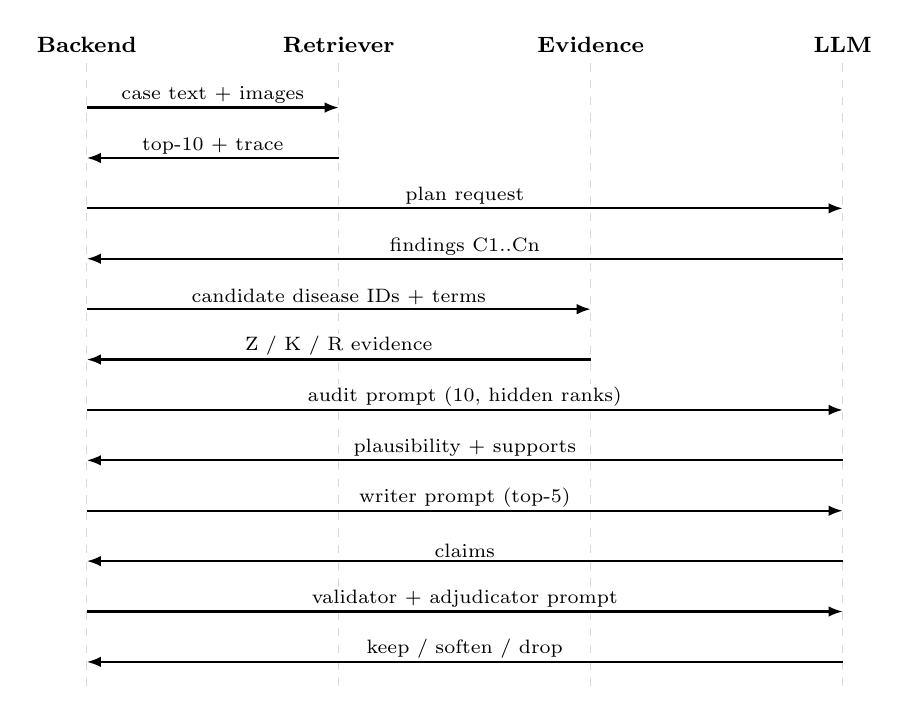
\begin{tikzpicture}[
  x=1cm,y=0.8cm,
  lifeline/.style={draw=rule,dashed},
  msg/.style={-{Latex[length=1.8mm]},thick},
  lab/.style={font=\scriptsize,fill=white,inner sep=1pt}
]
\node[font=\footnotesize\bfseries] (backend) at (0,0) {Backend};
\node[font=\footnotesize\bfseries] (ret) at (3.2,0) {Retriever};
\node[font=\footnotesize\bfseries] (ev) at (6.4,0) {Evidence};
\node[font=\footnotesize\bfseries] (llm) at (9.6,0) {LLM};
\foreach \x in {0,3.2,6.4,9.6} \draw[lifeline] (\x,-0.3) -- (\x,-10.2);
\draw[msg] (0,-1.0) -- node[lab,above]{case text + images} (3.2,-1.0);
\draw[msg] (3.2,-1.8) -- node[lab,above]{top-10 + trace} (0,-1.8);
\draw[msg] (0,-2.6) -- node[lab,above]{plan request} (9.6,-2.6);
\draw[msg] (9.6,-3.4) -- node[lab,above]{findings C1..Cn} (0,-3.4);
\draw[msg] (0,-4.2) -- node[lab,above]{candidate disease IDs + terms} (6.4,-4.2);
\draw[msg] (6.4,-5.0) -- node[lab,above]{Z / K / R evidence} (0,-5.0);
\draw[msg] (0,-5.8) -- node[lab,above]{audit prompt (10, hidden ranks)} (9.6,-5.8);
\draw[msg] (9.6,-6.6) -- node[lab,above]{plausibility + supports} (0,-6.6);
\draw[msg] (0,-7.4) -- node[lab,above]{writer prompt (top-5)} (9.6,-7.4);
\draw[msg] (9.6,-8.2) -- node[lab,above]{claims} (0,-8.2);
\draw[msg] (0,-9.0) -- node[lab,above]{validator + adjudicator prompt} (9.6,-9.0);
\draw[msg] (9.6,-9.8) -- node[lab,above]{keep / soften / drop} (0,-9.8);
\end{tikzpicture}
\caption{Per-case request sequence. Every arrow is a fixed step; there is no
model-controlled branching.}
\end{figure}

\begin{lstlisting}[caption={Per-case pseudocode (simplified)}]
ranked, trace = retriever.rank(case.text)          # frozen, top 10 + full scores
findings      = call_plan(case, candidates=ranked) # CALL 1
evidence      = fetch(ranked, findings)            # Z / K / R, no LLM
llm_only      = call_llm_only(case, findings, ranked)  # CALL 2b
audit         = call_audit(findings, evidence)     # CALL 2, ranks hidden
final         = sort_by(audit.plausibility, tie=retriever_position)
claims        = call_writer(final[:5], findings, evidence)  # CALL 3
claims        = validate(claims, findings, evidence)        # deterministic
claims        = call_adjudicate(claims, cited_text_only)    # CALL 4
return report(final, claims, llm_only, trace)
\end{lstlisting}

\subsection{Concurrency, caching, and resume}

Each case is independent. The reference run used four workers, matching four
server slots. Every case is checkpointed as
\code{cases/<CaseID>.json}. A checkpoint is reused only when both the pipeline
version and the served model id match. Switching models therefore recomputes
cleanly instead of mixing outputs.

The image caption cache is keyed by absolute image path; captions and failures are
both cached. The OptimusKG slice is cached per run. The retriever artifacts are
loaded once.

\subsection{LLM server contract}

Any llama.cpp OpenAI-compatible server works:
\begin{lstlisting}
POST {LLM_BASE}/chat/completions
{
  "model": "<discovered from /v1/models>",
  "messages": [...],
  "temperature": 0.0,
  "seed": 42,
  "max_tokens": 1400..2600,
  "stream": false,
  "response_format": {"type": "json_object"},
  "chat_template_kwargs": {"enable_thinking": false}
}
\end{lstlisting}
If the server rejects \code{response\_format} or \code{chat\_template\_kwargs}, the
client retries without them. Invalid JSON triggers one repair round. Each stage has
a deterministic fallback, so one failed call does not crash a case.

\section{Evaluation protocol}

\subsection{Sampling}

The evaluation uses a random sample of the test split, seed 42. The interim agent
results use the first 62 completed cases of the 100-case sample (the run was stopped
early). This is a deterministic prefix, not a hand-picked subset, but it is still a
single sample; confidence intervals are reported.

\subsection{Metrics}

\begin{itemize}[leftmargin=1.4em]
\item \textbf{MRR} over the full 1,464-disease catalog: mean of $1/\mathrm{rank}$
of the gold disease.
\item \textbf{Top-1, top-5, top-10}: fraction of cases whose gold is within the
cutoff.
\item \textbf{Delta}: per-case change in reciprocal rank, complete system minus
retrieval, with a 2,000-sample bootstrap 95\% CI.
\item \textbf{Plausibility separation}: AUROC of gold versus non-gold candidates
within the audited top-10.
\item \textbf{Citation validity}: deterministic validator pass rate.
\item \textbf{Evidence usefulness}: KG coverage, share of claims citing KG,
keep-or-soften rate for KG-citing versus ZebraMap-only claims, and retriever-term
verification rate.
\end{itemize}

\subsection{Retrieval reference}

The shipped retriever's full-test results are in Section~\ref{sec:retrieval-results}.
The live reference implementation was additionally checked on 100 sampled test
cases: its top-10 disease IDs matched the cached pipeline in every case.

\section{Agent-layer results (interim)}
\label{sec:agent-results}

\subsection{Setup}

Two local llama.cpp models were tested at temperature 0 with thinking disabled:

\begin{center}
\begin{tabular}{lll}
\toprule
Model & Cases & Role\\
\midrule
Groot-19B-A3B (Q4\_K\_M) & 4 & smoke test only\\
Gemma-4-E4B-it-qat (Q4\_K\_XL) & 62 & interim evaluation\\
\bottomrule
\end{tabular}
\end{center}

The 4-case Groot smoke test gave retrieval MRR 0.591, complete 0.633, LLM-only
0.558. It is too small to interpret and is included only for completeness.

\subsection{Gemma-4-E4B, 62 cases}

\begin{center}
\begin{tabular}{lrrrr}
\toprule
System & MRR & Top-1 & Top-5 & Top-10\\
\midrule
Retrieval alone & \textbf{0.4744} & \textbf{0.3871} & \textbf{0.5806} & 0.5968\\
LLM-only (no evidence) & 0.4202 & 0.3226 & 0.5323 & 0.5968\\
Complete system & 0.4199 & 0.2742 & 0.5484 & 0.5968\\
\bottomrule
\end{tabular}
\end{center}

Per-case delta (complete minus retrieval): \textbf{$-0.0545$} MRR, bootstrap 95\%
CI $[-0.1377, +0.0276]$; 8 wins, 14 losses, 40 ties. Top-5 rescued 1, lost 3.

\begin{center}
\begin{tabular}{lrrr}
\toprule
Gold retrieval rank & $n$ & Retrieval MRR & Complete MRR\\
\midrule
1 & 24 & 1.000 & 0.707\\
2--5 & 12 & 0.378 & \textbf{0.612}\\
6--10 & 1 & 0.167 & 1.000\\
$>$10 & 25 & 0.029 & 0.029\\
\bottomrule
\end{tabular}
\end{center}

\textbf{Interpretation.} The auditor is useful when the retriever is uncertain
(ranks 2--5) and harmful when the retriever is already correct. This is the classic
failure mode of an LLM reranker with a weak prior: it overweights textbook-looking
alternatives and demotes an obvious correct answer. A rank-prior blend or a
confidence gate on the retriever's top-1 margin is the natural next experiment.

\subsection{Explanation quality}

\begin{center}
\begin{tabular}{lr}
\toprule
Quantity & Value\\
\midrule
Claims & 630 (10.16 per case)\\
Validator pass rate & 56.98\%\\
Adjudication & keep 548, soften 41, drop 41\\
Support claims & 546 (86.7\%)\\
Claims citing OptimusKG & 121 (19.2\%)\\
KG coverage of audited candidates & 80.0\%\\
Audit evidence references & Z 352, K 88, R 521\\
\bottomrule
\end{tabular}
\end{center}

The dominant validator failure is a support claim that cites disease evidence but
no case finding (about 85\% of invalid claims). A smaller group (about 37 claims)
is candidate-label confusion: a claim written for candidate C cites \code{Z-I-*}.
The latter can be repaired deterministically from the evidence ID; the former
cannot, because attaching a finding after the fact would fabricate grounding.

\subsection{Qualitative examples}

\textbf{Rescued (rank 6 to 1): self-limited epilepsy with centrotemporal spikes.}
The retriever ranked West syndrome first. The auditor promoted the correct disease
(plausibility 75) and the writer produced well-cited claims, for example:
\begin{quote}\small
``EEG showed spike and slow waves in the right rolandic area during sleep [C7] and
[Z-F-2].''\\
``The patient experienced seizures accompanied by grunting after falling asleep
[C4] and [K-F-2].''\\
``Brain MRI and neurological exam were normal, excluding structural etiologies
[C8] and [Z-F-4].''
\end{quote}

\textbf{Harmed (rank 1 to 7): X-linked lymphoproliferative disease.}
The auditor demoted the gold to plausibility 40 because its retrieved ZebraMap
profile did not mention the case's CNS findings, and promoted CACH syndrome to 75.
The ranking change is evidence-faithful but clinically wrong. Its claims also
showed cross-candidate citation errors, which the validator caught.

\textbf{Lesson.} The evidence layer is doing real work; the weak point is the
auditor's calibration and citation discipline, not the retrieval or the evidence
fetching.

\section{Live deployment guide}

This section is written for the engineer building the chat frontend and backend.

\subsection{Recommended backend architecture}

\begin{center}
\begin{tabular}{ll}
\toprule
Component & Recommendation\\
\midrule
API & FastAPI (Python 3.13), async endpoints + SSE for progress\\
Queue & Redis + RQ or Celery; one job per case analysis\\
Session store & PostgreSQL for sessions/messages/reports; Redis for hot state\\
Weights & local files from \code{weights/retriever}; load once per process\\
LLM & llama.cpp server, OpenAI-compatible; one model per deployment\\
Object store & JSON reports per case (S3/MinIO or disk)\\
Observability & structured logs per stage, token counts, latency, validator rate\\
\bottomrule
\end{tabular}
\end{center}

The retriever is CPU-friendly. The LLM dominates latency. In the 62-case run,
Gemma-4-E4B averaged about 150 seconds per case serially at four workers, including
all five LLM calls. Retrieval alone is roughly one second per case on CPU.

\subsection{Session and chat-history model}

A conversation is a sequence of turns. Two turn types are enough:

\begin{itemize}[leftmargin=1.4em]
\item \code{analyze\_case}: the user submits a new case (text, optional images).
This triggers retrieval and the full explanation pipeline.
\item \code{follow\_up}: the user asks a question about the current report
(``why is disease B above C?'', ``show the evidence for claim 3''). This does
\emph{not} re-run retrieval. The backend answers from the stored report and can
call a compact follow-up prompt with the pinned evidence.
\end{itemize}

Store the following per session:
\begin{lstlisting}
session_id, created_at, model_id, prompt_version, retriever_version
turns: [{turn_id, type, user_text, case_hash, report_id, created_at}]
pinned_report: {top10, evidence, audit, claims, adjudication, trace}
\end{lstlisting}

Chat-history rules:
\begin{enumerate}[leftmargin=1.4em]
\item Never recompute retrieval for a follow-up unless the user edits the case.
\item Do not resend the full evidence on every follow-up. Store it once and pass
compact references (disease label, claim id, evidence ids).
\item Pin the model id and prompt version in the session. If the server model
changes, mark the session as stale and offer a re-run.
\item Cache by \code{sha256(case\_text + image\_hashes + model\_id + prompt\_version)}.
Identical submissions return the stored report.
\end{enumerate}

\subsection{API contract}

\begin{lstlisting}
POST /v1/sessions
  -> {session_id}

POST /v1/sessions/{id}/messages
  {type: "analyze_case", text: "...", images: [base64...]}
  -> {turn_id, job_id}                     # 202 Accepted

GET /v1/jobs/{job_id}/events               # text/event-stream
  event: stage   data: {"stage":"retrieved","progress":0.15}
  event: stage   data: {"stage":"planned","progress":0.30}
  event: stage   data: {"stage":"audited","progress":0.60}
  event: stage   data: {"stage":"written","progress":0.80}
  event: stage   data: {"stage":"adjudicated","progress":1.0}
  event: done    data: {"report_id":"..."}

GET /v1/reports/{report_id}
  {
    "case_id": "...",
    "retrieval": {"mrr": 1.0, "top10": [...]},
    "llm_only": {"order": [...], "metrics": {...}},
    "final_order": [{"rank":1,"disease_id":"758","name":"...","plausibility":82,
                     "retriever_rank":1}],
    "claims": [{"disease":"...","claim":"...","cites":["C2","Z-A-1"],
                "verdict":"keep","validator_ok":true}],
    "trace": {...}
  }

POST /v1/sessions/{id}/messages
  {type: "follow_up", text: "Why is CACH above XLP?"}
  -> {answer, cited_claims: [...], evidence_refs: [...]}
\end{lstlisting}

\subsection{Frontend requirements}

\begin{itemize}[leftmargin=1.4em]
\item Show the retriever order and the final order side by side, with arrows for
moved diseases. This makes the LLM's effect visible and auditable.
\item Show plausibility as a bar, not a percentage with false precision.
\item Render every claim with clickable citation chips. Clicking \code{Z-A-1} shows
the exact source sentence; clicking \code{C2} highlights the case span.
\item Show struck claims with a strikethrough and the adjudicator's reason.
\item Show the LLM-only baseline in a collapsible panel; it is a diagnostic, not a
recommendation.
\item Always show the disclaimer: research prototype, not a diagnostic device.
\end{itemize}

\subsection{Latency and scaling}

\begin{center}
\begin{tabular}{lr}
\toprule
Stage & Typical latency (7B-class local model, 4 slots)\\
\midrule
Retrieval (CPU) & $\sim$1 s\\
CALL 1 plan & 20--45 s\\
CALL 2b LLM-only & 8--12 s\\
CALL 2 audit (10 candidates) & 50--95 s\\
CALL 3 writer (top 5) & 20--45 s\\
CALL 4 adjudicator & 15--30 s\\
Total per case (serial) & 2--4 min\\
\bottomrule
\end{tabular}
\end{center}

For a live chat UI, stream stage events and keep the request asynchronous. If
interactive latency matters, run the retriever immediately, return the top-10, and
let explanations fill in progressively. A GPU-backed server or a smaller model
reduces the LLM share substantially.

\subsection{Model and prompt versioning}

The prompt version and model id are part of the cache key and the report. A change
to either invalidates stored explanations. The retriever version is separate; a
retriever change requires recomputing the candidate list and all downstream stages.
Do not mix reports produced under different versions in one evaluation table.

\subsection{Safety and governance}

\begin{itemize}[leftmargin=1.4em]
\item The system is a research prototype and must not be presented as a diagnostic
device.
\item Case text may contain identifiable information. Prefer local inference, avoid
logging raw text, and store only hashes plus the structured report when possible.
\item Evidence citations are the audit trail. Never display a claim without its
citations.
\item KG and profile evidence can be incomplete or outdated; absence of a finding
is not evidence of absence.
\item The LLM-only baseline exists to show what the model would say without
evidence; it should not be used for decisions.
\end{itemize}

\section{Reproducibility and artifact manifest}

\subsection{Environment}

Python 3.13, LightGBM 4.7.0, scikit-learn 1.9.1, NumPy 2.5.4, SciPy 1.18.1,
pandas 3.1.1, PyTorch 2.15.0+cpu, transformers 5.24.0, joblib 1.6.0, Tectonic
0.17.0. The LLM is served by llama.cpp. All retrieval training used CPU
LightGBM; captions use CPU PyTorch.

\subsection{Shipped weights}

\begin{center}
\begin{longtable}{llr}
\toprule
File & Role & Size\\
\midrule
\code{gbm\_v4\_shap8.txt} & production LambdaRank model, 8 features, 241 trees & 847 KB\\
\code{gbm\_v4\_140.txt} & full 140-feature LambdaRank alternative & 256 KB\\
\code{tfidf\_vectorizer.joblib} & 50k-feature 1--2 gram TF-IDF & 1.9 MB\\
\code{tfidf\_classifier.joblib} & SGD log-loss, 1,464 classes & 280 MB\\
\code{bow\_vectorizer\_mass80.pkl} & mass80 TF-IDF vectorizer & 1.8 MB\\
\code{bow\_centroids\_mass80.npz} & 1,464 L2-normalised centroids & 9.4 MB\\
\code{prune\_sets\_mass80.json} & 2,075 removed word forms & 92 KB\\
\code{svd32.joblib} & 32-component TruncatedSVD & 6.2 MB\\
\code{disease\_svd32.npy} & 1,464 x 32 disease SVD rows & 184 KB\\
\code{diseases.json} & catalog order and names & 125 KB\\
\code{retriever\_config.json} & fusion weights and metrics & 1 KB\\
\bottomrule
\end{longtable}
\end{center}

Catalog data:
\begin{center}
\begin{tabular}{llr}
\toprule
File & Role & Size\\
\midrule
\code{disease\_index.json} & id, name, index for 1,464 diseases & 167 KB\\
\code{augmented\_disease\_data.json} & full ZebraMap/Orphanet profiles & 9.5 MB\\
\code{optimuskg\_catalog.json} & phenotype/gene/parent slice, 1,244 diseases & 1.2 MB\\
\bottomrule
\end{tabular}
\end{center}

\subsection{Verification performed}

\begin{itemize}[leftmargin=1.4em]
\item Saved GBM boosters reload and reproduce the reported val/test metrics.
\item The SVD refit reproduces the cached case and disease SVD features exactly
(max absolute difference 0).
\item The live reference retriever matches the cached top-10 on all 100 sampled
test cases used for verification.
\item The full-test retrieval metrics were reproduced from the cached benchmark
artifacts (MRR 0.4960, top-5 0.6199, top-10 0.6848). The raw-text live reference
matched the cached top-10 on all 100 sampled verification cases.
\end{itemize}

\subsection{Quick start for the backend engineer}

\begin{lstlisting}
from reference_retriever import Retriever

ret = Retriever("weights/retriever")
out = ret.rank(case_text, k=10)
for row in out["top"]:
    print(row["rank"], row["disease_id"], row["name"], row["score"])
\end{lstlisting}

For the full explanation layer, run \code{glassbox\_pipeline.py} with
\code{--no-caption} during development, then enable captions for the final product.
Point \code{LLM\_BASE} at the local server. The pipeline writes per-case JSON and a
report, which the API can serve directly.

\section{Limitations and next steps}

\begin{enumerate}[leftmargin=1.4em]
\item \textbf{Agent ranking is not yet an improvement.} The evidence-conditioned
auditor loses more on correct top-1 cases than it gains on ranks 2--5. Validate a
retrieval-prior blend or a confidence gate before exposing LLM reordering as the
default.
\item \textbf{Citation discipline is model-dependent.} Gemma-4-E4B produced 57\%
valid claims; the larger Groot model produced roughly 90\% in the smoke test.
Model choice matters as much as prompt design.
\item \textbf{OptimusKG evidence is sparse for some diseases.} Coverage is 85\% of
the catalog; absence of a KG link is reported, never fabricated.
\item \textbf{Image captions are weak for non-radiology images.} BLIP-ROCO is a
radiology captioner; ophthalmology, dermatology, and histopathology captions can be
wrong. Treat modality metadata as authoritative.
\item \textbf{The 62-case agent sample is a prefix of one random sample.} Report
confidence intervals and do not over-interpret small deltas.
\item \textbf{Top-10 is fixed by design.} Any future system that lets the LLM
promote candidates outside the top-10 needs a new evaluation that reports the
expanded candidate set honestly.
\end{enumerate}

\key{Recommended next experiments} (in order):
\begin{enumerate}[leftmargin=1.4em]
\item Rank-prior blend: $S' = \mathrm{plausibility} + \lambda(1/\mathrm{retriever\ rank})$
or a reciprocal-rank fusion, tuned on validation, reported on test.
\item Confidence gate: only let the LLM reorder when the retriever top-1 margin is
below a threshold.
\item Claim repair: infer the candidate label from evidence IDs and drop
disease-only support claims at write time.
\item Stronger citation model: rerun the writer with a larger model while keeping
the same evidence, to separate model capacity from evidence quality.
\end{enumerate}

\appendix
\section{Record schema}

Each per-case JSON contains:
\begin{lstlisting}
{
  "pipeline_version": "glassbox-v2",
  "llm_model": "...",
  "case_id": "...",
  "gold_disease_id": "...",
  "gold_disease_name": "...",
  "retriever": {"system": "fusion_v4_shap8", "metrics": {...}, "top10": [...]},
  "images": [{"image_id","modality","subtype","caption","caption_model"}],
  "findings": [{"id","text","type","quote","quote_verified","source"}],
  "evidence": {"A": {"disease_id","name","z":[...],"k":[...],
                     "kg_available","trace":{...}}},
  "audit": {"ok": true, "candidates": [...]},
  "candidates": [{"label","audit_label","disease_id","name",
                  "plausibility","retriever_rank","final_rank"}],
  "final_order": [...],
  "final_metrics": {"mrr","top1","top5","top10","rank"},
  "claims": [{"candidate","disease","kind","claim","cites",
              "validator_ok","validator_errors","adjudication"}],
  "llm_only_baseline": {"order":[...],"top5":[...],"metrics":{...}},
  "elapsed_s": 0.0
}
\end{lstlisting}

\section{File manifest}

\begin{lstlisting}
handoff/
  README.md
  docs/architecture.tex
  docs/architecture.pdf
  weights/retriever/
    gbm_v4_shap8.txt
    gbm_v4_140.txt
    tfidf_vectorizer.joblib
    tfidf_classifier.joblib
    tfidf_config.json
    bow_vectorizer_mass80.pkl
    bow_centroids_mass80.npz
    prune_sets_mass80.json
    svd32.joblib
    disease_svd32.npy
    diseases.json
    retriever_config.json
  weights/catalog/
    disease_index.json
    augmented_disease_data.json
    optimuskg_catalog.json
  code/
    glassbox_pipeline.py
    reference_retriever.py
    live_backend_example.py
    prompts.md
  results/
    retrieval_full_test.json
    agent_interim_62.json
  SHA256SUMS
\end{lstlisting}

\end{document}
